% Options for packages loaded elsewhere
\PassOptionsToPackage{unicode}{hyperref}
\PassOptionsToPackage{hyphens}{url}
%
\documentclass[
  a4paper,
  oneside]{book}

\usepackage{amsmath,amssymb}
\usepackage{iftex}
\ifPDFTeX
  \usepackage[T1]{fontenc}
  \usepackage[utf8]{inputenc}
  \usepackage{textcomp} % provide euro and other symbols
\else % if luatex or xetex
  \usepackage{unicode-math}
  \defaultfontfeatures{Scale=MatchLowercase}
  \defaultfontfeatures[\rmfamily]{Ligatures=TeX,Scale=1}
\fi
\usepackage{lmodern}
\ifPDFTeX\else  
    % xetex/luatex font selection
\fi
% Use upquote if available, for straight quotes in verbatim environments
\IfFileExists{upquote.sty}{\usepackage{upquote}}{}
\IfFileExists{microtype.sty}{% use microtype if available
  \usepackage[]{microtype}
  \UseMicrotypeSet[protrusion]{basicmath} % disable protrusion for tt fonts
}{}
\makeatletter
\@ifundefined{KOMAClassName}{% if non-KOMA class
  \IfFileExists{parskip.sty}{%
    \usepackage{parskip}
  }{% else
    \setlength{\parindent}{0pt}
    \setlength{\parskip}{6pt plus 2pt minus 1pt}}
}{% if KOMA class
  \KOMAoptions{parskip=half}}
\makeatother
\usepackage{xcolor}
\setlength{\emergencystretch}{3em} % prevent overfull lines
\setcounter{secnumdepth}{5}
% Make \paragraph and \subparagraph free-standing
\ifx\paragraph\undefined\else
  \let\oldparagraph\paragraph
  \renewcommand{\paragraph}[1]{\oldparagraph{#1}\mbox{}}
\fi
\ifx\subparagraph\undefined\else
  \let\oldsubparagraph\subparagraph
  \renewcommand{\subparagraph}[1]{\oldsubparagraph{#1}\mbox{}}
\fi

\usepackage{color}
\usepackage{fancyvrb}
\newcommand{\VerbBar}{|}
\newcommand{\VERB}{\Verb[commandchars=\\\{\}]}
\DefineVerbatimEnvironment{Highlighting}{Verbatim}{commandchars=\\\{\}}
% Add ',fontsize=\small' for more characters per line
\usepackage{framed}
\definecolor{shadecolor}{RGB}{241,243,245}
\newenvironment{Shaded}{\begin{snugshade}}{\end{snugshade}}
\newcommand{\AlertTok}[1]{\textcolor[rgb]{0.68,0.00,0.00}{#1}}
\newcommand{\AnnotationTok}[1]{\textcolor[rgb]{0.37,0.37,0.37}{#1}}
\newcommand{\AttributeTok}[1]{\textcolor[rgb]{0.40,0.45,0.13}{#1}}
\newcommand{\BaseNTok}[1]{\textcolor[rgb]{0.68,0.00,0.00}{#1}}
\newcommand{\BuiltInTok}[1]{\textcolor[rgb]{0.00,0.23,0.31}{#1}}
\newcommand{\CharTok}[1]{\textcolor[rgb]{0.13,0.47,0.30}{#1}}
\newcommand{\CommentTok}[1]{\textcolor[rgb]{0.37,0.37,0.37}{#1}}
\newcommand{\CommentVarTok}[1]{\textcolor[rgb]{0.37,0.37,0.37}{\textit{#1}}}
\newcommand{\ConstantTok}[1]{\textcolor[rgb]{0.56,0.35,0.01}{#1}}
\newcommand{\ControlFlowTok}[1]{\textcolor[rgb]{0.00,0.23,0.31}{#1}}
\newcommand{\DataTypeTok}[1]{\textcolor[rgb]{0.68,0.00,0.00}{#1}}
\newcommand{\DecValTok}[1]{\textcolor[rgb]{0.68,0.00,0.00}{#1}}
\newcommand{\DocumentationTok}[1]{\textcolor[rgb]{0.37,0.37,0.37}{\textit{#1}}}
\newcommand{\ErrorTok}[1]{\textcolor[rgb]{0.68,0.00,0.00}{#1}}
\newcommand{\ExtensionTok}[1]{\textcolor[rgb]{0.00,0.23,0.31}{#1}}
\newcommand{\FloatTok}[1]{\textcolor[rgb]{0.68,0.00,0.00}{#1}}
\newcommand{\FunctionTok}[1]{\textcolor[rgb]{0.28,0.35,0.67}{#1}}
\newcommand{\ImportTok}[1]{\textcolor[rgb]{0.00,0.46,0.62}{#1}}
\newcommand{\InformationTok}[1]{\textcolor[rgb]{0.37,0.37,0.37}{#1}}
\newcommand{\KeywordTok}[1]{\textcolor[rgb]{0.00,0.23,0.31}{#1}}
\newcommand{\NormalTok}[1]{\textcolor[rgb]{0.00,0.23,0.31}{#1}}
\newcommand{\OperatorTok}[1]{\textcolor[rgb]{0.37,0.37,0.37}{#1}}
\newcommand{\OtherTok}[1]{\textcolor[rgb]{0.00,0.23,0.31}{#1}}
\newcommand{\PreprocessorTok}[1]{\textcolor[rgb]{0.68,0.00,0.00}{#1}}
\newcommand{\RegionMarkerTok}[1]{\textcolor[rgb]{0.00,0.23,0.31}{#1}}
\newcommand{\SpecialCharTok}[1]{\textcolor[rgb]{0.37,0.37,0.37}{#1}}
\newcommand{\SpecialStringTok}[1]{\textcolor[rgb]{0.13,0.47,0.30}{#1}}
\newcommand{\StringTok}[1]{\textcolor[rgb]{0.13,0.47,0.30}{#1}}
\newcommand{\VariableTok}[1]{\textcolor[rgb]{0.07,0.07,0.07}{#1}}
\newcommand{\VerbatimStringTok}[1]{\textcolor[rgb]{0.13,0.47,0.30}{#1}}
\newcommand{\WarningTok}[1]{\textcolor[rgb]{0.37,0.37,0.37}{\textit{#1}}}

\providecommand{\tightlist}{%
  \setlength{\itemsep}{0pt}\setlength{\parskip}{0pt}}\usepackage{longtable,booktabs,array}
\usepackage{calc} % for calculating minipage widths
% Correct order of tables after \paragraph or \subparagraph
\usepackage{etoolbox}
\makeatletter
\patchcmd\longtable{\par}{\if@noskipsec\mbox{}\fi\par}{}{}
\makeatother
% Allow footnotes in longtable head/foot
\IfFileExists{footnotehyper.sty}{\usepackage{footnotehyper}}{\usepackage{footnote}}
\makesavenoteenv{longtable}
\usepackage{graphicx}
\makeatletter
\def\maxwidth{\ifdim\Gin@nat@width>\linewidth\linewidth\else\Gin@nat@width\fi}
\def\maxheight{\ifdim\Gin@nat@height>\textheight\textheight\else\Gin@nat@height\fi}
\makeatother
% Scale images if necessary, so that they will not overflow the page
% margins by default, and it is still possible to overwrite the defaults
% using explicit options in \includegraphics[width, height, ...]{}
\setkeys{Gin}{width=\maxwidth,height=\maxheight,keepaspectratio}
% Set default figure placement to htbp
\makeatletter
\def\fps@figure{htbp}
\makeatother
% definitions for citeproc citations
\NewDocumentCommand\citeproctext{}{}
\NewDocumentCommand\citeproc{mm}{%
  \begingroup\def\citeproctext{#2}\cite{#1}\endgroup}
\makeatletter
 % allow citations to break across lines
 \let\@cite@ofmt\@firstofone
 % avoid brackets around text for \cite:
 \def\@biblabel#1{}
 \def\@cite#1#2{{#1\if@tempswa , #2\fi}}
\makeatother
\newlength{\cslhangindent}
\setlength{\cslhangindent}{1.5em}
\newlength{\csllabelwidth}
\setlength{\csllabelwidth}{3em}
\newenvironment{CSLReferences}[2] % #1 hanging-indent, #2 entry-spacing
 {\begin{list}{}{%
  \setlength{\itemindent}{0pt}
  \setlength{\leftmargin}{0pt}
  \setlength{\parsep}{0pt}
  % turn on hanging indent if param 1 is 1
  \ifodd #1
   \setlength{\leftmargin}{\cslhangindent}
   \setlength{\itemindent}{-1\cslhangindent}
  \fi
  % set entry spacing
  \setlength{\itemsep}{#2\baselineskip}}}
 {\end{list}}
\usepackage{calc}
\newcommand{\CSLBlock}[1]{\hfill\break\parbox[t]{\linewidth}{\strut\ignorespaces#1\strut}}
\newcommand{\CSLLeftMargin}[1]{\parbox[t]{\csllabelwidth}{\strut#1\strut}}
\newcommand{\CSLRightInline}[1]{\parbox[t]{\linewidth - \csllabelwidth}{\strut#1\strut}}
\newcommand{\CSLIndent}[1]{\hspace{\cslhangindent}#1}

\usepackage{unicode-math}%
\setmathfont{XITS Math}%
\usepackage{fontspec}%
\setmainfont[Ligatures ={Common, TeX}, Scale=1, RawFeature={+cpsp}]{XITS} 
%Numbers={Lining,Proportional},Ligatures ={Common, TeX},RawFeature={+tnum,+cpsp,+frac},
\setsansfont[RawFeature={+cpsp},Scale=MatchLowercase]{Helvetica Neue}%
\setmonofont[Scale=0.85]{Source Code Pro}%

\usepackage[a4paper,%
margin=2.5cm,%
bottom=3cm,%
top=3cm]{geometry}%
\usepackage{afterpage}% for "\afterpage"
\usepackage{xcolor}%
\definecolor{dundeeblue}{HTML}{4365E2}%
\usepackage{pagecolor}% With option pagecolor={somecolor or none}
%% For nice tables
\usepackage{booktabs}%
\usepackage{longtable}%
\usepackage{array}%
\usepackage{multirow}%
\usepackage{wrapfig}%
\usepackage{float}%
\usepackage{colortbl}%
%\usepackage{pdflscape}%
\usepackage{tabu}%
%\usepackage{threeparttable}%
%\usepackage{threeparttablex}%
%\usepackage[normalem]{ulem}%
\usepackage{makecell}%
%% Wrap long output lines
\usepackage{listings}%
\lstset{breaklines=true}%
\usepackage{enumitem}%
\setlist[description]{style=nextline}%
%% For nice info boxes
\usepackage{fontawesome5}%
\usepackage{awesomebox}%
\usepackage{siunitx}%
\newcolumntype{d}{S[table-format=3.2]}%
\renewcommand{\bibname}{References}%
%\usepackage[colorlinks]{hyperref}%

\usepackage{titling}%
%\setlength{\droptitle}{8cm}
\pretitle{\newpagecolor{dundeeblue}\afterpage{\restorepagecolor} \vfill \begin{flushleft}
\fontsize{68pt}{62pt} \color{white}\sffamily\bfseries\selectfont }
\posttitle{\end{flushleft}}

\preauthor{\vspace{2.5cm} \begin{flushleft} \fontsize{18pt}{14pt} \color{white}\sffamily\selectfont}
\postauthor{$\quad\bullet\quad$ehall001@dundee.ac.uk\end{flushleft}}

\predate{\begin{flushleft} \fontsize{18pt}{14pt} \color{white}\sffamily\selectfont}
\postdate{\\ \vspace{1cm}\includegraphics[width=10cm]{assets/images/rev_logo.pdf}\end{flushleft}}

%%% BEGIN SHORTCUTS
\DeclareMathOperator{\E}{\mathbf{E}}%
\DeclareMathOperator{\Var}{Var}%
\DeclareMathOperator{\Cov}{Cov}%
\DeclareMathOperator{\corr}{corr}%
\DeclareMathOperator{\sd}{sd}%
\newcommand{\se}{\mathsf{se}}%
\newcommand{\gt}{>}%
\newcommand{\lt}{<}%
%%% END SHORTCUTS

%% Change chapter to Topic
\makeatletter
\renewcommand{\@chapapp}{Topic}
\makeatother

\usepackage{tocbibind}



\usepackage{booktabs}
\usepackage{longtable}
\usepackage{array}
\usepackage{multirow}
\usepackage{wrapfig}
\usepackage{float}
\usepackage{colortbl}
\usepackage{pdflscape}
\usepackage{tabu}
\usepackage{threeparttable}
\usepackage{threeparttablex}
\usepackage[normalem]{ulem}
\usepackage{makecell}
\usepackage{xcolor}
\makeatletter
\@ifpackageloaded{tcolorbox}{}{\usepackage[skins,breakable]{tcolorbox}}
\@ifpackageloaded{fontawesome5}{}{\usepackage{fontawesome5}}
\definecolor{quarto-callout-color}{HTML}{909090}
\definecolor{quarto-callout-note-color}{HTML}{0758E5}
\definecolor{quarto-callout-important-color}{HTML}{CC1914}
\definecolor{quarto-callout-warning-color}{HTML}{EB9113}
\definecolor{quarto-callout-tip-color}{HTML}{00A047}
\definecolor{quarto-callout-caution-color}{HTML}{FC5300}
\definecolor{quarto-callout-color-frame}{HTML}{acacac}
\definecolor{quarto-callout-note-color-frame}{HTML}{4582ec}
\definecolor{quarto-callout-important-color-frame}{HTML}{d9534f}
\definecolor{quarto-callout-warning-color-frame}{HTML}{f0ad4e}
\definecolor{quarto-callout-tip-color-frame}{HTML}{02b875}
\definecolor{quarto-callout-caution-color-frame}{HTML}{fd7e14}
\makeatother
\makeatletter
\@ifpackageloaded{caption}{}{\usepackage{caption}}
\AtBeginDocument{%
\ifdefined\contentsname
  \renewcommand*\contentsname{Table of contents}
\else
  \newcommand\contentsname{Table of contents}
\fi
\ifdefined\listfigurename
  \renewcommand*\listfigurename{List of Figures}
\else
  \newcommand\listfigurename{List of Figures}
\fi
\ifdefined\listtablename
  \renewcommand*\listtablename{List of Tables}
\else
  \newcommand\listtablename{List of Tables}
\fi
\ifdefined\figurename
  \renewcommand*\figurename{Figure}
\else
  \newcommand\figurename{Figure}
\fi
\ifdefined\tablename
  \renewcommand*\tablename{Table}
\else
  \newcommand\tablename{Table}
\fi
}
\@ifpackageloaded{float}{}{\usepackage{float}}
\floatstyle{ruled}
\@ifundefined{c@chapter}{\newfloat{codelisting}{h}{lop}}{\newfloat{codelisting}{h}{lop}[chapter]}
\floatname{codelisting}{Listing}
\newcommand*\listoflistings{\listof{codelisting}{List of Listings}}
\usepackage{amsthm}
\theoremstyle{definition}
\newtheorem{definition}{Definition}[chapter]
\theoremstyle{definition}
\newtheorem{example}{Example}[chapter]
\theoremstyle{definition}
\newtheorem{exercise}{Exercise}[chapter]
\theoremstyle{plain}
\newtheorem{theorem}{Theorem}[chapter]
\theoremstyle{remark}
\AtBeginDocument{\renewcommand*{\proofname}{Proof}}
\newtheorem*{remark}{Remark}
\newtheorem*{solution}{Solution}
\newtheorem{refremark}{Remark}[chapter]
\newtheorem{refsolution}{Solution}[chapter]
\makeatother
\makeatletter
\makeatother
\makeatletter
\@ifpackageloaded{caption}{}{\usepackage{caption}}
\@ifpackageloaded{subcaption}{}{\usepackage{subcaption}}
\makeatother
\ifLuaTeX
  \usepackage{selnolig}  % disable illegal ligatures
\fi
\usepackage{bookmark}

\IfFileExists{xurl.sty}{\usepackage{xurl}}{} % add URL line breaks if available
\urlstyle{same} % disable monospaced font for URLs
\hypersetup{
  pdftitle={MA22004 - Statistics II},
  pdfauthor={Dr Eric Hall},
  hidelinks,
  pdfcreator={LaTeX via pandoc}}

\title{MA22004 - Statistics II}
\author{Dr Eric Hall}
\date{2024-09-02}

\begin{document}
\frontmatter
\maketitle

\renewcommand*\contentsname{Table of contents}
{
\setcounter{tocdepth}{2}
\tableofcontents
}
\mainmatter
\chapter*{Welcome}\label{welcome}
\addcontentsline{toc}{chapter}{Welcome}

\markboth{Welcome}{Welcome}

Welcome to MA22004 at the University of Dundee.

This module covers the basics of statistical inference. This document
contains the content. The appendix contains a list of curated content
for your to investigate.

\section*{About your instructor}\label{about-your-instructor}
\addcontentsline{toc}{section}{About your instructor}

\markright{About your instructor}

Hi, folks!

\includegraphics{assets/images/Eric_Hall_small.jpg}

I'm Eric---your instructor for MA22004 this semester. I am a new Baxter
Fellow in Applied Mathematics at Dundee, and my research focuses on
uncertainty quantification and predictive modelling.

Originally from the US, I graduated from the University of Pennsylvania
with a BA in Mathematics. I wrote my PhD in Probability and Stochastic
Analysis at the University of Edinburgh. Math and stats have opened up
some exciting doors for me, and I've had the opportunity to undertake
postdoctoral work at KTH Stockholm, the University of Massachusetts
Amherst, and RWTH Aachen University. I'm very excited to be at Dundee
and back in Scotland. I'm even more excited to be teaching you
statistics this semester!

\begin{center}\rule{0.5\linewidth}{0.5pt}\end{center}

These notes are available at
\href{https://dundeemath.github.io/MA22004/}{dundeemath.github.io/MA22004/}
and also as a PDF (visit the page and click on the PDF icon to
download).

\section*{Licence}\label{licence}
\addcontentsline{toc}{section}{Licence}

\markright{Licence}

\includegraphics{index_files/mediabag/88x31.png}

This work is licensed under a
\href{http://creativecommons.org/licenses/by-nc/4.0/}{Creative Commons
Attribution-NonCommercial 4.0 International License}.

\part{Module Introduction}

\chapter*{Lab Guide \{.unnumbered
-\#labs=``\,``\}}\label{lab-guide-.unnumbered--labs}
\addcontentsline{toc}{chapter}{Lab Guide \{.unnumbered -\#labs=``\,``\}}

\markboth{Lab Guide \{.unnumbered -\#labs=``\,``\}}{Lab Guide
\{.unnumbered -\#labs=``\,``\}}

You will learn about the statistical programming language \texttt{R} and
the software RStudio by working through seven interactive lab tutorials
and completing lab reports. The lab reports should answer the exercise
questions at the end of each tutorial.

Tutorials and all associated materials (templates, data sets, further
instructions, etc.) are available as an \texttt{R} package at the GitHub
repository \texttt{dundeemath/MA22004labs} (i.e.,
\url{https://github.com/dundeemath/MA22004labs}).

Instructions on how to install and access the interactive lab tutorials
can be found at:

\begin{itemize}
\tightlist
\item
  \url{https://dundeemath.github.io/MA22004labs/}.
\end{itemize}

The following section contains details about lab reports.

\chapter*{Writing Lab Reports \{.unnumbered
-\#writing=``\,``\}}\label{writing-lab-reports-.unnumbered--writing}
\addcontentsline{toc}{chapter}{Writing Lab Reports \{.unnumbered
-\#writing=``\,``\}}

\markboth{Writing Lab Reports \{.unnumbered -\#writing=``\,``\}}{Writing
Lab Reports \{.unnumbered -\#writing=``\,``\}}

\section*{Assessment Criteria}\label{w-assess}
\addcontentsline{toc}{section}{Assessment Criteria}

\markright{Assessment Criteria}

There are seven interactive lab tutorials with accompanying exercises.
Each lab tutorial specifies how marks are allocated across the exercises
(a maximum of 20 marks available for each lab report).

\begin{importantblock}
Marks are awarded for both \textbf{content} and \textbf{presentation}.

\end{importantblock}

\section*{Content}\label{w-content}
\addcontentsline{toc}{section}{Content}

\markright{Content}

Please work through the interactive tutorial for each lab. Your lab
report should answer the exercises found at the end of each tutorial.

\section*{Presentation}\label{w-present}
\addcontentsline{toc}{section}{Presentation}

\markright{Presentation}

Please use R Markdown to create your lab report. Further instructions on
using R Markdown for creating \emph{reproducible} lab reports that
combine data analysis and text can be found in Lab 1.

\subsection*{Plots}\label{w-plots}
\addcontentsline{toc}{subsection}{Plots}

Plots should be neat and legible, with appropriate aesthetic elements.
Please use \texttt{ggplot} for creating plots and visualisations. Each
plot should be annotated with titles, axis labels, and legends as
appropriate. Plot aesthetics should be distinguished, e.g.~using colours
or line styles that are identified using a legend. Important data points
and coordinates should be annotated using labels.

\subsection*{Mathematical formulas}\label{w-math}
\addcontentsline{toc}{subsection}{Mathematical formulas}

Mathematical formulas should follow the same style rules as the lecture
notes. Formulas can be included in R Markdown documents using \LaTeX{}
syntax. There should be appropriate spacing around operators and equals
signs, e.g.~\(a + b = c\). For punctuation, formulas are treated as part
of the text, so they often need to end with a full stop or comma.
Important formulas can appear ``displayed'' on their own line (with line
spacing above and below them), e.g. {[}A=πr\^{}2,.{]}

\subsection*{Structure}\label{w-structure}
\addcontentsline{toc}{subsection}{Structure}

Structure should be logical and clear. Organise your writing with
suitable headings and sub-headings. For example, provide a solution to
each exercise under its own heading.

\subsection*{Writing}\label{w-eng}
\addcontentsline{toc}{subsection}{Writing}

Writing should follow the usual rules of good written English, including
writing complete sentences and paragraphs that get to the point quickly.
Your tone and language should be similar to lecture notes or scientific
journal articles. Formal writing does not require unnecessary words,
long words or monotonous use of passive voice. I will reward concise and
clear communication, so please do not write, ``Upon carefully analysing
the aforementioned equations, the following mathematical solution was
found,'' when ``The solution is'' conveys the same thing.

\subsection*{Formatting}\label{w-format}
\addcontentsline{toc}{subsection}{Formatting}

Formatting should rely on the \emph{MA22004 Lab Report} template. This
is available in the \texttt{MA22004labs} package, and further
instructions can be found in Lab 1.

\part{Lecture Notes}

\chapter*{Preliminaries}\label{preliminaries}
\addcontentsline{toc}{chapter}{Preliminaries}

\markboth{Preliminaries}{Preliminaries}

This section contains a list of abbreviations, comment on notation, and
a (very quick) review of probability.

\section*{Abbreviations}\label{abbreviations}
\addcontentsline{toc}{section}{Abbreviations}

\markright{Abbreviations}

In Table~\ref{tbl-abbrev} we list abbreviations used throughout these
lecture notes. These abbreviations are pretty standdard and you might
encounter them outside the module in other references.

\begin{longtable}[t]{ll}

\caption{\label{tbl-abbrev}Commonly used abbreviations.}

\tabularnewline

\toprule
Abbreviation & Expanded\\
\midrule
\endfirsthead
\multicolumn{2}{@{}l}{\textit{(continued)}}\\
\toprule
Abbreviation & Expanded\\
\midrule
\endhead

\endfoot
\bottomrule
\endlastfoot
\cellcolor{gray!10}{pdf} & \cellcolor{gray!10}{probability density function}\\
cdf & cumulative distribution function\\
\cellcolor{gray!10}{rv} & \cellcolor{gray!10}{random variable}\\
iid & independent and identically distributed\\
\cellcolor{gray!10}{obs} & \cellcolor{gray!10}{observations}\\
\addlinespace
CI & confidence interval\\
\cellcolor{gray!10}{df} & \cellcolor{gray!10}{degrees of freedom}\\*

\end{longtable}

\section*{Notation}\label{notation}
\addcontentsline{toc}{section}{Notation}

\markright{Notation}

Uppercase roman letters, e.g., \(X\), will typically denote random
variables (rvs); lower case letters, e.g., \(x\), will represent a
particular value (observation) of a rv. Rvs have probability
distributions. Distributions are typically characterised by
\emph{parameters} that describe population characteristics. In the
present module, we will adopt the (frequentists) view that parameters
are fixed real numbers that are often unknown and must be estimated from
data. Statistical inference is a tool that will help us to do this.

\begin{tcolorbox}[enhanced jigsaw, colframe=quarto-callout-warning-color-frame, breakable, toprule=.15mm, bottomrule=.15mm, title=\textcolor{quarto-callout-warning-color}{\faExclamationTriangle}\hspace{0.5em}{Warning}, arc=.35mm, opacityback=0, left=2mm, opacitybacktitle=0.6, bottomtitle=1mm, toptitle=1mm, titlerule=0mm, rightrule=.15mm, colback=white, colbacktitle=quarto-callout-warning-color!10!white, coltitle=black, leftrule=.75mm]

Statistical models comprise both rvs and parameters. Be careful not to
confuse them!

\end{tcolorbox}

For a random variable \(X\) that has a distribution \(F\) depending on a
parameter \(\theta\), we will write \(X \sim F(\theta)\).

\begin{tcolorbox}[enhanced jigsaw, colframe=quarto-callout-warning-color-frame, breakable, toprule=.15mm, bottomrule=.15mm, title=\textcolor{quarto-callout-warning-color}{\faExclamationTriangle}\hspace{0.5em}{Warning}, arc=.35mm, opacityback=0, left=2mm, opacitybacktitle=0.6, bottomtitle=1mm, toptitle=1mm, titlerule=0mm, rightrule=.15mm, colback=white, colbacktitle=quarto-callout-warning-color!10!white, coltitle=black, leftrule=.75mm]

We write \(X \sim F\) to indicate \(X\) has distribution \(F\), not
``\(X\) is approximately \(F\)''!

\end{tcolorbox}

\section*{Sample space, events,
probabilities}\label{sample-space-events-probabilities}
\addcontentsline{toc}{section}{Sample space, events, probabilities}

\markright{Sample space, events, probabilities}

A \emph{sample space} \(\Omega\) is a set of possible outcomes of an
experiment. Points \(\omega \in \Omega\) are \emph{sample outcomes} or
realizations. Subsets \(A \subset \Omega\) are called \emph{events}.

\begin{example}[Sample
space]\protect\hypertarget{exm-sample-space}{}\label{exm-sample-space}

Consider an experiment where we measure the petal widths from a randomly
sampled cyclamen flowers. Before we observe the petal width, there is
uncertainty that we can model using a sample space of events. The sample
space is \(\Omega = (0, \infty)\), since measurements of length should
be positive (practically, the lengths will have a finite size, too).
Each \(\omega \in \Omega\) is a measurement of petal width for a
cyclamen flower. Consider an event \(A = (5, 12]\); this is the event
that the petal width is larger than \(5\) but less than or equal to
\(12\). Remember, we use probability to model uncertainty \emph{before}
we observe the petal width --- after we take a measurement, the petal
width is no longer uncertain (we have collected a statistic).

\end{example}

As sample spaces and events are described using sets, we recall the
following notations, definitions, and laws about set theory. Let \(A\),
\(B\), and \(A_1, A_2, \dots\) be events in a sample space \(\Omega\).

\begin{itemize}
\item
  complement: \(A^c = \{ \omega \in \Omega: \omega \notin A\}\).
\item
  null event: \(\emptyset = \Omega^c\).
\item
  intersection:
  \(A \cap B = \{\omega \in \Omega : \omega \in A \text{ and } \omega \in B\}\).
  In particular, for \(A_1, A_2, \dots\), then
  \[\bigcap_{i=1}^\infty A_i = \{\omega \in \Omega : \omega \in A_i \text{ for all } i \}\,.\]
\item
  difference:
  \(A \setminus B = \{\omega \in \Omega : \omega \in A, \omega \notin B\}\).
\item
  size: \(|A|\) denotes the number of elements in \(A\).
\item
  disjoint: \(A_i \cap A_j = \emptyset\), for \(i\neq j\).
\item
  partition: disjoint \(A_1, A_2, \dots\) such that
  \(\bigcup_{i=1}^\infty A_i = \Omega\).
\item
  indicator:
  \(I_A(\omega) = I(\omega \in A) = \{1 \text{ if } \omega \in A; 0 \text{ if } \omega \notin A\}\).
\item
  monotone increasing: \(A_1 \subset A_2 \subset \dots\) and define
  limit \[\lim_{n \to \infty}A_n = \bigcup_{i=1}^\infty A_i\,.\]
\item
  monotone decreasing: \(A_1 \supset A_2 \supset \dots\) and define
  limit \[\lim_{n \to \infty} A_n = \bigcap_{i=1}^\infty A_i\,.\]
\item
  distributive laws: \[A\cap (B\cup C) = (A\cap B) \cup (A \cap C)\,,\]
  \[A\cup(B\cap C) = (A \cup B) \cap (A\cup C)\,.\]
\item
  De Morgan's laws: \[(A \cap B)^c = A^c \cup B^c\,,\]
  \[(A\cup B)^c = A^c \cap B^c\,.\]
\end{itemize}

We assign probabilities to events in our sample space.

\begin{definition}[Probability
distribution]\protect\hypertarget{def-prob}{}\label{def-prob}

A probability distribution is a function \(P : \Omega \to \mathbf{R}\)
satisfying three axioms: 1. \(P(A) \geq 0\) for every
\(A \subset \Omega\) (positivity), 2. \(P(\Omega) = 1\) (totality), 3.
if \(A_1, A_2, \dots\) are disjoint subsets of \(\Omega\), then
\[P(\cup_{i=1}^\infty A_i) = \sum_{i=1}^\infty P(A_i)\,.\]

\end{definition}

\begin{tcolorbox}[enhanced jigsaw, colframe=quarto-callout-tip-color-frame, breakable, toprule=.15mm, bottomrule=.15mm, title=\textcolor{quarto-callout-tip-color}{\faLightbulb}\hspace{0.5em}{Tip}, arc=.35mm, opacityback=0, left=2mm, opacitybacktitle=0.6, bottomtitle=1mm, toptitle=1mm, titlerule=0mm, rightrule=.15mm, colback=white, colbacktitle=quarto-callout-tip-color!10!white, coltitle=black, leftrule=.75mm]

We can interpret \(P(A)\) as representing:

\begin{itemize}
\tightlist
\item
  \textbf{frequency}, i.e., the long-run proportion of times \(A\) is
  true (the \emph{frequentist perspective}),
\item
  \textbf{degrees of belief}, i.e, as a measure of the observer's
  strength of belief that \(A\) is true (the \emph{Bayesian
  perspective}).
\end{itemize}

\end{tcolorbox}

\begin{theorem}[PIE]\protect\hypertarget{thm-pie}{}\label{thm-pie}

The principal of inclusion-exclusion,
\[P(A\cup B) = P(A) + P(B) - P(A\cap B)\,.\]

\end{theorem}

Theorem~\ref{thm-pie} follows from the definition of a probability
distributions and facts about set theory.

\begin{definition}[Probability of an
event]\protect\hypertarget{def-prob-finite}{}\label{def-prob-finite}

For events \(A\) from finite sample spaces \(\Omega\), we assign
probabilities according to: \[P(A) = \frac{|A|}{|\Omega|} \,.\]

\end{definition}

For finite sample spaces, we assign probabilities according to their
long-run frequency of occurring. For an event \(A\), this is the ratio
of the size of \(A\) (number of ways \(A\) can happen) to the size of
\(\Omega\) (number of total outcomes).

\begin{definition}[Independent
events]\protect\hypertarget{def-indep}{}\label{def-indep}

Events \(A\) and \(B\) are independent, i.e.,
\(A \perp \!\!\! \perp B\), iff \(P(A\cap B) = P(A)P(B)\).

\end{definition}

That is, events \(A\) and \(B\) are independent if and only if the
probability of \(A\) and \(B\) occurring is equal to the the probability
\(A\) occurring times the probability of \(B\) occurring.

\begin{definition}[Conditional
probability]\protect\hypertarget{def-cond-prob}{}\label{def-cond-prob}

If \(P(B) > 0\), then \[P(A \mid B) = \frac{P(A \cap B)}{P(B)}\,.\]

\end{definition}

Note that:

\begin{itemize}
\tightlist
\item
  \(P(\cdot \mid B)\) satisfies the axioms of probability, for fixed
  \(B\),
\item
  in general, \(P(A \mid \cdot)\) is not a probability for fixed \(A\),
  and,
\item
  in general, \(P(A\mid B) \neq P(B \mid A)\).
\end{itemize}

\begin{theorem}[Bayes
Theorem]\protect\hypertarget{thm-bayes}{}\label{thm-bayes}

Let events \(A_1, \dots, A_k\) partition \(\Omega\), with
\(P(A_i) > 0\).

If \(P(B) > 0\), then
\[P(A_i \mid B) = \frac{P(B\mid A_i) P(A_i)}{\sum_j P(B \mid A_j) P(A_j)}\,.\]

\end{theorem}

Generally, it is not feasible to assign probabilities to \emph{all}
subsets of \(\Omega\) (e.g., if \Omega is infinite). In that case, we
restrict to our attention to a \(\sigma\)-algebra \(\mathcal{A}\) (also
called, \(\sigma\)-field), which is a collection of sets satisfying: 1.
\(\mathbf{E}mptyset \in \mathcal{A}\), 2. if
\(A_1, A_2, \dots, \in \mathcal{A}\) then
\(\cup_{i = 1}^\infty A_i \in \mathcal{A}\), 3.
\(A\in \mathcal{A} \implies A^c \in \mathcal{A}\).

Sets in \(\mathcal{A}\) are said to be \emph{measurable} and
\((\Omega, \mathcal{A})\) is a measure space. If \(P\) is a probability
defined on \(\mathcal{A}\), then \((\Omega, \mathcal{A}, P)\) is called
a \emph{probability space}.

E.g., when \(\Omega \mathbf{E}quiv \mathbf{R}\), we take \(\mathcal{A}\)
to be the smallest \(\sigma\)-field containing all open subsets of
\(\mathbf{R}\), which is called the Borel \(\sigma\)-field. If you find
these details interesting, take: MA42008 Mathematical Statistics!

\section*{Random variables}\label{random-variables}
\addcontentsline{toc}{section}{Random variables}

\markright{Random variables}

\begin{tcolorbox}[enhanced jigsaw, colframe=quarto-callout-note-color-frame, breakable, toprule=.15mm, bottomrule=.15mm, title=\textcolor{quarto-callout-note-color}{\faInfo}\hspace{0.5em}{Note}, arc=.35mm, opacityback=0, left=2mm, opacitybacktitle=0.6, bottomtitle=1mm, toptitle=1mm, titlerule=0mm, rightrule=.15mm, colback=white, colbacktitle=quarto-callout-note-color!10!white, coltitle=black, leftrule=.75mm]

How do we link sample spaces and events to data?

\end{tcolorbox}

We use random variables to link sample spaces and events to data.

\begin{definition}[Random
variables]\protect\hypertarget{def-rv}{}\label{def-rv}

A random variable (rv) is a mapping \(X : \Omega \to \mathbf{R}\) that
maps \(\omega \in \Omega \mapsto X(\omega)\).

\end{definition}

\begin{example}[]\protect\hypertarget{exm-rv-1}{}\label{exm-rv-1}

Consider a coin flipping experiment where you flip a fair coin eight
times. Let \(X\) be the number of heads in the sequence. If three heads
occur, e.g., \(\omega = HTTTTTHH\), then \(X(\omega) = 3\).

\end{example}

\begin{example}[]\protect\hypertarget{exm-rv-2}{}\label{exm-rv-2}

Consider an experiment where you draw a point a random from the unit
disk. Then \(\Omega = \{(x,y) : x^2 + y^2 \leq 1\}\) and a typical
outcome will be the pair \(\omega = (x,y)\). Some random variables to
consider are \(X(\omega) = x\), \(Y(\omega) = y\), \(Z(\omega) = x+y\),
and \(W(\omega) = \sqrt{x^2 + y^2}\).

\end{example}

\begin{definition}[Assigning probabilities to
rvs]\protect\hypertarget{def-prob-rv}{}\label{def-prob-rv}

Given \(X\) and \(A \subset \mathbf{R}\), we define
\[X^{-1}(A) = \{\omega \in \Omega : X(\omega) \in A\}\] and let
\[P(X \in A) = P(X^{-1}(A)) = P(\{\omega \in \Omega : X(\omega) \in A\})\,,\]
e.g.,
\(P(X=x) = P(X^{-1}(x)) = P(\{\omega \in \Omega : X(\omega) = x\})\).

\end{definition}

\begin{tcolorbox}[enhanced jigsaw, colframe=quarto-callout-warning-color-frame, breakable, toprule=.15mm, bottomrule=.15mm, title=\textcolor{quarto-callout-warning-color}{\faExclamationTriangle}\hspace{0.5em}{Warning}, arc=.35mm, opacityback=0, left=2mm, opacitybacktitle=0.6, bottomtitle=1mm, toptitle=1mm, titlerule=0mm, rightrule=.15mm, colback=white, colbacktitle=quarto-callout-warning-color!10!white, coltitle=black, leftrule=.75mm]

\(X\) denotes a rv and \(x\) denotes a particular value of \(X\). You
would never write \(P(X)\), would you!?

\end{tcolorbox}

\begin{example}[]\protect\hypertarget{exm-rv-3}{}\label{exm-rv-3}

Consider a coin flipping experiment where you flip a fair coin twice.
Let \(X\) be the number of heads. Then
\[P(X=0) = P(\{TT\}) = \frac{1}{4}\,,\]
\[P(X=1) = P(\{HT\} \cup \{TH\}) = P(\{HT\}) + P(\{TH\}) = \frac{1}{2}\,,\]
\[P(X=2) = P(\{HH\}) = \frac{1}{4}\,.\]

\end{example}

\begin{definition}[]\protect\hypertarget{def-cdf}{}\label{def-cdf}

\#\#~Cdf

The cumulative distribution function (cdf),
\(F_X:\mathbf{R} \to [0,1]\), is defined by \(F_X(x) = P(X \leq x)\).

\end{definition}

\begin{Shaded}
\begin{Highlighting}[]
\NormalTok{x }\OtherTok{\textless{}{-}} \FunctionTok{c}\NormalTok{(}\DecValTok{0}\NormalTok{, }\DecValTok{0}\NormalTok{, }\DecValTok{1}\NormalTok{, }\DecValTok{1}\NormalTok{, }\DecValTok{2}\NormalTok{, }\DecValTok{2}\NormalTok{)}
\NormalTok{y }\OtherTok{\textless{}{-}} \FunctionTok{c}\NormalTok{(}\DecValTok{0}\NormalTok{, }\FloatTok{0.25}\NormalTok{, }\FloatTok{0.25}\NormalTok{, }\FloatTok{0.75}\NormalTok{, }\FloatTok{0.75}\NormalTok{, }\DecValTok{1}\NormalTok{)}
\NormalTok{b }\OtherTok{\textless{}{-}} \FunctionTok{c}\NormalTok{(}\StringTok{"o"}\NormalTok{, }\StringTok{"c"}\NormalTok{, }\StringTok{"o"}\NormalTok{, }\StringTok{"c"}\NormalTok{, }\StringTok{"o"}\NormalTok{, }\StringTok{"c"}\NormalTok{)}
\NormalTok{dat }\OtherTok{\textless{}{-}} \FunctionTok{data.frame}\NormalTok{(x, y, b)}
\NormalTok{dat}\SpecialCharTok{$}\NormalTok{b }\OtherTok{\textless{}{-}} \FunctionTok{factor}\NormalTok{(dat}\SpecialCharTok{$}\NormalTok{b)}
\NormalTok{dat }\SpecialCharTok{|\textgreater{}} \FunctionTok{ggplot}\NormalTok{(}\FunctionTok{aes}\NormalTok{(x, y, }\AttributeTok{shape =}\NormalTok{ b)) }\SpecialCharTok{+}
  \FunctionTok{geom\_point}\NormalTok{(}\AttributeTok{size =}\NormalTok{ lsz }\SpecialCharTok{+}\NormalTok{ lsz}\SpecialCharTok{*}\DecValTok{2}\NormalTok{, }\AttributeTok{color =} \StringTok{"\#E41A1C"}\NormalTok{) }\SpecialCharTok{+}
  \FunctionTok{geom\_segment}\NormalTok{(}\FunctionTok{aes}\NormalTok{(}\AttributeTok{x =} \DecValTok{0}\NormalTok{, }\AttributeTok{y =} \DecValTok{0}\NormalTok{, }\AttributeTok{xend =} \SpecialCharTok{{-}}\DecValTok{1}\NormalTok{, }\AttributeTok{yend =} \DecValTok{0}\NormalTok{), }\AttributeTok{arrow =} \FunctionTok{arrow}\NormalTok{(}\AttributeTok{length =} \FunctionTok{unit}\NormalTok{(}\FloatTok{0.25}\SpecialCharTok{*}\NormalTok{lsz, }\StringTok{"cm"}\NormalTok{)), }\AttributeTok{linewidth =}\NormalTok{ lsz, }\AttributeTok{color =} \StringTok{"\#E41A1C"}\NormalTok{) }\SpecialCharTok{+}
  \FunctionTok{geom\_segment}\NormalTok{(}\FunctionTok{aes}\NormalTok{(}\AttributeTok{x =} \DecValTok{0}\NormalTok{, }\AttributeTok{y =} \FloatTok{0.25}\NormalTok{, }\AttributeTok{xend =} \DecValTok{1}\NormalTok{, }\AttributeTok{yend =} \FloatTok{0.25}\NormalTok{), }\AttributeTok{linewidth =}\NormalTok{ lsz, }\AttributeTok{color =} \StringTok{"\#E41A1C"}\NormalTok{) }\SpecialCharTok{+}
  \FunctionTok{geom\_segment}\NormalTok{(}\FunctionTok{aes}\NormalTok{(}\AttributeTok{x =} \DecValTok{1}\NormalTok{, }\AttributeTok{y =} \FloatTok{0.75}\NormalTok{, }\AttributeTok{xend =} \DecValTok{2}\NormalTok{, }\AttributeTok{yend =} \FloatTok{0.75}\NormalTok{), }\AttributeTok{linewidth =}\NormalTok{ lsz, }\AttributeTok{color =} \StringTok{"\#E41A1C"}\NormalTok{) }\SpecialCharTok{+}
  \FunctionTok{geom\_segment}\NormalTok{(}\FunctionTok{aes}\NormalTok{(}\AttributeTok{x =} \DecValTok{2}\NormalTok{, }\AttributeTok{y =} \DecValTok{1}\NormalTok{, }\AttributeTok{xend =} \DecValTok{3}\NormalTok{, }\AttributeTok{yend =} \DecValTok{1}\NormalTok{), }\AttributeTok{arrow =} \FunctionTok{arrow}\NormalTok{(}\AttributeTok{length =} \FunctionTok{unit}\NormalTok{(}\FloatTok{0.25}\SpecialCharTok{*}\NormalTok{lsz, }\StringTok{"cm"}\NormalTok{)), }\AttributeTok{linewidth =}\NormalTok{ lsz, }\AttributeTok{color =} \StringTok{"\#E41A1C"}\NormalTok{) }\SpecialCharTok{+}
  \FunctionTok{geom\_vline}\NormalTok{(}\FunctionTok{aes}\NormalTok{(}\AttributeTok{xintercept =} \DecValTok{0}\NormalTok{)) }\SpecialCharTok{+}
  \FunctionTok{geom\_hline}\NormalTok{(}\FunctionTok{aes}\NormalTok{(}\AttributeTok{yintercept =} \DecValTok{0}\NormalTok{)) }\SpecialCharTok{+}
 \FunctionTok{scale\_shape\_manual}\NormalTok{(}\AttributeTok{values =} \FunctionTok{c}\NormalTok{(}\DecValTok{19}\NormalTok{, }\DecValTok{1}\NormalTok{)) }\SpecialCharTok{+}
  \FunctionTok{theme}\NormalTok{(}\AttributeTok{axis.line.x =} \FunctionTok{element\_blank}\NormalTok{(), }
        \AttributeTok{axis.text.x =} \FunctionTok{element\_blank}\NormalTok{(),}
        \AttributeTok{axis.ticks.x =} \FunctionTok{element\_blank}\NormalTok{()) }\SpecialCharTok{+}
 \FunctionTok{guides}\NormalTok{(}\AttributeTok{shape =} \StringTok{"none"}\NormalTok{) }\SpecialCharTok{+} 
 \FunctionTok{labs}\NormalTok{(}\AttributeTok{x =} \FunctionTok{TeX}\NormalTok{(}\StringTok{"$x$"}\NormalTok{), }\AttributeTok{y =} \FunctionTok{TeX}\NormalTok{(}\StringTok{"$F\_X(x)$"}\NormalTok{)) }\SpecialCharTok{+}\NormalTok{ theme\_ur}
\end{Highlighting}
\end{Shaded}

\begin{figure}[H]

\centering{

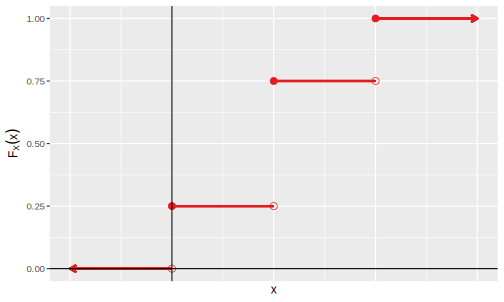
\includegraphics{00-prelim_files/figure-pdf/fig-eg-cdf-coin-flip-plot-1.pdf}

}

\caption{\label{fig-eg-cdf-coin-flip-plot}The cdf for the two coin flip
example.}

\end{figure}%

Note that a cdf completely determines the distribution of a random
variable.

\begin{theorem}[]\protect\hypertarget{thm-cdf-determines-dist}{}\label{thm-cdf-determines-dist}

Let \(X\) have cdf \(F\) and \(Y\) have cdf \(G\). If \(F(x) = G(x)\)
for all \(x\), then \(P(X \in A)= P(Y \in A) \forall A \in \mathbf{R}\).

\end{theorem}

\begin{theorem}[Properties of
cdfs]\protect\hypertarget{thm-cdf-properties}{}\label{thm-cdf-properties}

\(F : \mathbf{R} \to [0,1]\) is a cdf for some \(P\) iff,

\begin{enumerate}
\def\labelenumi{\arabic{enumi}.}
\tightlist
\item
  \(F\) is nondecreasing (i.e.,
  \(x_1 < x_2 \implies F(x_1) \leq F(x_2)\)),
\item
  \(F\) is normalized to \([0,1]\) (i.e.,
  \(\lim_{x \to -\infty} F(x) = 0\) and
  \(\lim_{x \to \infty} F(x) = 1\)),
\item
  \(F\) is right-continuous (i.e., \(F(x) = F(x^*) \forall x\) where
  \(F(x^*) = \lim_{y > x; y \to x} F(y)\)).
\end{enumerate}

\end{theorem}

For a rv \(X\) we say \(X\) is \emph{discrete} if it assumes at most a
\emph{countable} number of (discrete) values. For a discrete sample
space, the collection of all probabilities of \(X(\omega)\) gives us a
probability distribution.

\begin{definition}[Pmf]\protect\hypertarget{def-pmf}{}\label{def-pmf}

A pdf for a discrete rv \(X\) is \(f_X(x) = P(X = x)\). Since this
density function places a ``point mass'' at each \(x\), it is sometimes
referred to as a probability mass function (pmf).

\end{definition}

\begin{Shaded}
\begin{Highlighting}[]
\NormalTok{x }\OtherTok{\textless{}{-}} \FunctionTok{c}\NormalTok{(}\DecValTok{0}\NormalTok{, }\DecValTok{1}\NormalTok{, }\DecValTok{2}\NormalTok{)}
\NormalTok{y }\OtherTok{\textless{}{-}} \FunctionTok{c}\NormalTok{(}\FloatTok{0.25}\NormalTok{, }\FloatTok{0.50}\NormalTok{, }\FloatTok{0.25}\NormalTok{)}
\NormalTok{b }\OtherTok{\textless{}{-}} \FunctionTok{c}\NormalTok{(}\StringTok{"a"}\NormalTok{, }\StringTok{"a"}\NormalTok{, }\StringTok{"a"}\NormalTok{)}
\NormalTok{dat }\OtherTok{\textless{}{-}} \FunctionTok{data.frame}\NormalTok{(x, y, b)}
\NormalTok{dat}\SpecialCharTok{$}\NormalTok{b }\OtherTok{\textless{}{-}} \FunctionTok{factor}\NormalTok{(dat}\SpecialCharTok{$}\NormalTok{b)}
\NormalTok{dat }\SpecialCharTok{|\textgreater{}} \FunctionTok{ggplot}\NormalTok{(}\FunctionTok{aes}\NormalTok{(x, y, }\AttributeTok{color =}\NormalTok{ b, }\AttributeTok{fill =}\NormalTok{ b)) }\SpecialCharTok{+}
  \FunctionTok{geom\_bar}\NormalTok{(}\AttributeTok{stat =} \StringTok{"identity"}\NormalTok{, }\AttributeTok{linewidth =}\NormalTok{lsz) }\SpecialCharTok{+}
  \FunctionTok{geom\_hline}\NormalTok{(}\AttributeTok{yintercept =} \DecValTok{0}\NormalTok{) }\SpecialCharTok{+} \FunctionTok{geom\_vline}\NormalTok{(}\AttributeTok{xintercept =} \SpecialCharTok{{-}}\DecValTok{1}\NormalTok{) }\SpecialCharTok{+}
 \FunctionTok{guides}\NormalTok{(}\AttributeTok{fill =} \StringTok{"none"}\NormalTok{, }\AttributeTok{color =} \StringTok{"none"}\NormalTok{) }\SpecialCharTok{+} 
 \FunctionTok{labs}\NormalTok{(}\AttributeTok{x =} \FunctionTok{TeX}\NormalTok{(}\StringTok{"$x\_i$"}\NormalTok{), }\AttributeTok{y =} \FunctionTok{TeX}\NormalTok{(}\StringTok{"$f\_X(x\_i) = P(X(}\SpecialCharTok{\textbackslash{}\textbackslash{}}\StringTok{omega) = x\_i)$"}\NormalTok{)) }\SpecialCharTok{+}\NormalTok{ theme\_ur}
\end{Highlighting}
\end{Shaded}

\begin{figure}[H]

\centering{

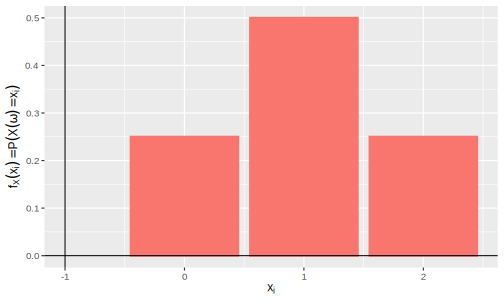
\includegraphics{00-prelim_files/figure-pdf/fig-eg-pmf-histogram-1.pdf}

}

\caption{\label{fig-eg-pmf-histogram}The histogram (pmf) for the two
coin flip example.}

\end{figure}%

Note, from the axioms of probability, that the pdf for a discrete random
variable therefore satisfies \(f(x) \geq 0\),
\(\forall x \in \mathbf{R}\) and \(\sum_i f(x_i) = 1\).

A rv \(X\) is \emph{continuous} if there exists a continuous function
\(f_X\) such that, 1. \(f_X(x) \geq 0 \forall x\), 2.
\(\int_{-\infty}^\infty f_X(x) dx = 1\) and 3.
\(P(a < X < b) = \int_a^b f_X(x) dx\), for \(a\leq b\).

\begin{definition}[Pdf]\protect\hypertarget{def-pdf}{}\label{def-pdf}

A \(f_X\) satisfying the three properties above is a pdf for the
continous rv \(X\).

\end{definition}

\begin{tcolorbox}[enhanced jigsaw, colframe=quarto-callout-warning-color-frame, breakable, toprule=.15mm, bottomrule=.15mm, title=\textcolor{quarto-callout-warning-color}{\faExclamationTriangle}\hspace{0.5em}{Warning}, arc=.35mm, opacityback=0, left=2mm, opacitybacktitle=0.6, bottomtitle=1mm, toptitle=1mm, titlerule=0mm, rightrule=.15mm, colback=white, colbacktitle=quarto-callout-warning-color!10!white, coltitle=black, leftrule=.75mm]

If \(X\) is continuous, then \(P(X = x) = 0\) for every \(x\). That is,
\[ 
P(a \leq X \leq b) = P(a < X \leq b) = P(a \leq X < b) = P(a < X < b),.
\]

\end{tcolorbox}

The cdf is related to the pdf by the derivative (difference). If \(X\)
is continuous: \[ F_X(x) = P(X \leq x) = \int_{-\infty}^x f_X(t) dt\]
and \(f_X(x) = F_X^\prime(x)\) at all \(x\) at which \(F_X\) is
differentiable. (Likewise, if \(X\) is discrete, then we replace the
integral with a sum
\(F_X(x) = P(X \leq x) = \sum_{x_i \leq x} f_X(x_i)\).)

\begin{definition}[Quantile
function]\protect\hypertarget{def-quantile}{}\label{def-quantile}

Let \(X\) be a rv with cdf \(F\). The inverse cdf, or quantile function,
is defined by \[F^{-1}(q) = \inf \{x : F(x) > q\}\] for \(q \in [0,1]\).
If \(F\) is monotonic increasing and continuous then \(F^{-1}(q)\) is
the unique real number \(x\) such that \(F(x) = q\).

\end{definition}

Some quantiles get used more than others (and therefore get names).
Important quantiles include, \(F^{-1}(\frac{1}{4})\) is the first
quantile, \(F^{-1}(\frac{1}{2})\) is the median, and
\(F^{-1}(\frac{3}{4})\) is the third quantile.

\begin{definition}[Equality in
distribution]\protect\hypertarget{def-equal-dist}{}\label{def-equal-dist}

We say \(X\) and \(Y\) are equal in distribution, \(X \equiv Y\), if
\(F_X(x) = F_Y(x)\) for all \(x\).

\end{definition}

\begin{tcolorbox}[enhanced jigsaw, colframe=quarto-callout-important-color-frame, breakable, toprule=.15mm, bottomrule=.15mm, title=\textcolor{quarto-callout-important-color}{\faExclamation}\hspace{0.5em}{Important}, arc=.35mm, opacityback=0, left=2mm, opacitybacktitle=0.6, bottomtitle=1mm, toptitle=1mm, titlerule=0mm, rightrule=.15mm, colback=white, colbacktitle=quarto-callout-important-color!10!white, coltitle=black, leftrule=.75mm]

Note that equality in distribution does not mean that the random
variables are the same. Rather, probability statements are the same.

Suppose \(P(X = 1) = P(X = -1) = \frac{1}{2}\). Let \(Y = -X\). Then
\(P(Y = 1) = P(Y = -1) = \frac{1}{2}\). Thus, \(X \mathbf{E}quiv Y\),
but \(X\) and \(Y\) are not equal; in fact, \(P(X = Y) = 0\).

\end{tcolorbox}

We sometimes consider more than one random variable, taken to together.
This leads to the concept of a joint and marginal densities.

\begin{definition}[Joint
pdf]\protect\hypertarget{def-joint-pdf}{}\label{def-joint-pdf}

A joint pdf for \((X,Y)\) satisfies

\begin{enumerate}
\def\labelenumi{\arabic{enumi}.}
\tightlist
\item
  \(f(x,y) \geq 0\) \(\forall x,y\),
\item
  \(\iint_{-\infty}^\infty f(x,y) dx dy = 1\),
\item
  for \(A \in \mathbf{R}\times \mathbf{R}\),
  \(P((X,Y) \in A) = \iint_A f(x,y) dx dy\).
\end{enumerate}

\end{definition}

\begin{definition}[Joint
cdf]\protect\hypertarget{def-joint-cdf}{}\label{def-joint-cdf}

A joint cdf is given by \(F(x,y) = P(X\leq x, Y\leq y)\).

\end{definition}

\begin{definition}[marginal
pdf]\protect\hypertarget{def-marginals}{}\label{def-marginals}

For \(X,Y\) with joint pdf \(f(x,y)\), we define the marginals for \(X\)
and \(Y\) as \(f_X(x) \int f(x,y) dy\) and \(f_Y(y) = \int f(x,y) dx\),
respectively.

\end{definition}

We also have a notion of independence for rvs.

\begin{definition}[Independence of
rvs]\protect\hypertarget{def-indep-rv}{}\label{def-indep-rv}

Rvs \(X\) and \(Y\) are independent if
\(P(X \in A, Y \in B) = P(X \in A) P(Y \in B)\).

\end{definition}

\begin{theorem}[]\protect\hypertarget{thm-pdf-indep-rv}{}\label{thm-pdf-indep-rv}

Let \(X,Y\) have joint \(f_{XY}\). Then \(X\) and \(Y\) are independent
iff \(f_{XY} = f_X \cdot f_Y\) for all \(x,y\).

\end{theorem}

If \(X_1, \dots X_n\) are independent and each as the same marginal
distribution with cdf \(F\), we say \(X_1, \dots, X_n\) are iid and
write \(X_1, \dots, X_n \sim F\) iid. We also write
\(X_1, \dots, X_n \sim f\) if \(F\) has corresponding density \(f\),
when no confusion arises.

\begin{definition}[Random
sample]\protect\hypertarget{def-sample}{}\label{def-sample}

\(X_1, \dots, X_n \sim F\) iid is a random sample of size \(n\) from a
distribution \(F\).

\end{definition}

We also consider the expected value of a rv.

\begin{definition}[Expectation]\protect\hypertarget{def-expected-value}{}\label{def-expected-value}

For a discrete rv \(X\) with possible outcomes \(x_1, x_2, \dots\) and
corresponding probabilities \(p_1, p_2, \dots\), the expectation is
defined by \[\mathbf{E}[X] = \sum_{i=1}^\infty x_i p_i\,.\]

For a continuous rv \(X\) with pdf \(f\), the expectation is defined by
\[\mathbf{E}[X] = \int_{-\infty}^{\infty} x f(x) dx\,.\]

\end{definition}

For both discrete and continuous rvs, we refer to various statistics
relating to expected values as moments of the distribution.

\begin{definition}[\(n\)-th raw
moment]\protect\hypertarget{def-raw-moments}{}\label{def-raw-moments}

For a rv \(X\), the \(n\)-th raw moment is given by \(\mathbf{E}[X^n]\).

\end{definition}

\begin{definition}[\(n\)-th central
moment]\protect\hypertarget{def-central-moments}{}\label{def-central-moments}

For a rv \(X\) with \(\mu = \mathbf{E}[X]\), the \(n\)-th central moment
is defined as \(\mathbf{E}[(X-\mu)^n]\).

\end{definition}

The \emph{mean} of a distribution is the first raw moment. The
\emph{variance} of a distribution is the second central moment.

\begin{table}

\caption{\label{tbl-moments}First three moments for a rv \(X\) with mean
\(\mu = \mathbf{E}[X]\).}

\begin{minipage}{0.50\linewidth}

\subcaption{\label{tbl-raw-moments}Raw moments}

\centering{

\begin{tabular}{cc}
\toprule
Expression & Name\\
\midrule
\(\mathbf{E}[X]\) & first (raw) moment\\
\(\mathbf{E}[X^2]\) & second (raw) moment\\
\(\mathbf{E}[X^3]\) & third (raw) moment\\
\bottomrule
\end{tabular}

}

\end{minipage}%
%
\begin{minipage}{0.50\linewidth}

\subcaption{\label{tbl-central-moments}Central moments}

\centering{

\begin{tabular}{cc}
\toprule
Expression & Name\\
\midrule
\(\mathbf{E}[(X - \mu)]\) & first central moment\\
\(\mathbf{E}[(X - \mu)^2]\) & second central moment\\
\(\mathbf{E}[(X - \mu)^3]\) & third central moment\\
\bottomrule
\end{tabular}

}

\end{minipage}%

\end{table}%

\chapter{Sampling distributions}\label{sec-sampling-distributions}

A \textbf{statistic} is a quantity that can be calculated from sample
data. Before observing data, a statistic is an unknown quantity and is,
therefore, a rv.

\begin{definition}[statistic]\protect\hypertarget{def-statistic}{}\label{def-statistic}

Let \(X_1, \dots, X_n\) be observable rvs and let \(g\) be an arbitrary
real-valued function of \(n\) random variables. The rv
\(T = g(X_1, \dots, X_n)\) is a \textbf{statistic}.

\end{definition}

We refer to the probability distribution for a statistic as a
\textbf{sampling distribution}. The sampling distribution illustrates
how the statistic will vary across \emph{possible} sample data. The
sampling distribution contains information about the values a statistic
is likely to assume and how likely it is to assume those values
\emph{prior to observing data}.

\begin{definition}[sampling
distribution]\protect\hypertarget{def-sampling-dist}{}\label{def-sampling-dist}

Suppose rvs \(X_1, \dots, X_n\) are a random sample from \(F(\theta)\),
a distribution depending a parameter \(\theta\) whose value is uknown.
Let the rv \(T = g(X_1, \dots, X_n, \theta)\) be a function of
\(X_1, \dots, X_n\) and (possibly) \(\theta\). The distribution of \(T\)
(given \(\theta\)) is the \textbf{sampling distribution} of \(T\).

\end{definition}

The sampling distribution of \(T\) is derived from the distribution of
the random sample. Often we will be interested in a statistic \(T\) that
is an estimator for a parameter \(\theta\) (that is, \(T\) will not
depend on \(\theta\)).

In what follows, we review several special families of distributions
that are widely used in probability and statistics. These special
families of distributions will be indexed by one or parameters.

\section{Uniform distribution}\label{uniform-distribution}

The uniform distribution places equal on uniform weight on the items
being sampled.

\begin{definition}[uniform
distribution]\protect\hypertarget{def-uniform-dist}{}\label{def-uniform-dist}

A continuous rv \(X\) has a \textbf{uniform distribution} on \([a,b]\)
with \(a<b\), if \(X\) has pdf \[
 f(x; a,b) = \frac{1}{b-a}\,, 
 \quad a < x < b\,,
\] or zero otherwise. We write \(X \sim \mathsf{Unif}(a,b)\).

\end{definition}

Note \(a\) and \(b\) are parameters.

\begin{exercise}[]\protect\hypertarget{exr-uniform}{}\label{exr-uniform}

As an exercise, derive the cdf using the definition. Derive a formula
for the mean and variance in terms of the parameters \(a\) and \(b\).

\end{exercise}

\section{Normal distribution}\label{sec-normal-distribution}

Normal distributions play an important role in probability and
statistics as they describe many natural phenomena. For instance, the
Central Limit Theorem tells us that the sample mean of a large random
sample (size \(m\)) of rvs with mean \(\mu\) and variance \(\sigma^2\)
is approximately normal in distribution with mean \(\mu\) and variance
\(\sigma^2/m\).

\begin{definition}[Normal or Gaussian
distribution]\protect\hypertarget{def-normal-dist}{}\label{def-normal-dist}

A continuous rv \(X\) has a \textbf{normal distribution} with parameters
\(\mu\) and \(\sigma^2\), where \(-\infty < \mu < \infty\) and
\(\sigma > 0\), if \(X\) has pdf \[
 f(x; \mu, \sigma) = \frac{1}{\sqrt{2 \pi} \sigma}e^{-(x-\mu)^2/(2\sigma^2)}\,, 
 \quad -\infty < x < \infty \,.
\] We write \(X \sim \mathsf{N}(\mu, \sigma^2)\).

\end{definition}

For \(X\sim \mathsf{N}(\mu,\sigma^2)\), it can be shown that
\(\E(X) = \mu\) and \(\Var(X) = \sigma^2\), that is, \(\mu\) is the
\emph{mean} and \(\sigma^2\) is the \emph{variance} of \(X\). The pdf
forms a bell-shaped curve that is symmetric about \(\mu\). The value
\(\sigma\) (\emph{standard deviation}) is the distance from \(\mu\) to
the inflection points of the curve. Thus, the distribution's position
(location) and spread depend on \(\mu\) and \(\sigma\).

\begin{verbatim}
Warning: Using `size` aesthetic for lines was deprecated in ggplot2 3.4.0.
i Please use `linewidth` instead.
\end{verbatim}

\begin{figure}[H]

{\centering 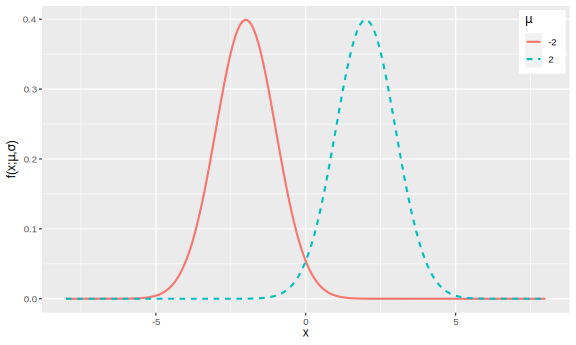
\includegraphics{01-sampling-distributions_files/figure-pdf/normals-diff-mean-1.pdf}

}

\caption{The pdfs of two normal rvs, \(X_1 \sim \mathsf{N}(-2, 1)\) and
\(X_2 \sim \mathsf{N}(2, 1)\), with \emph{different means} and the same
standard deviations.}

\end{figure}%

\begin{figure}[H]

{\centering 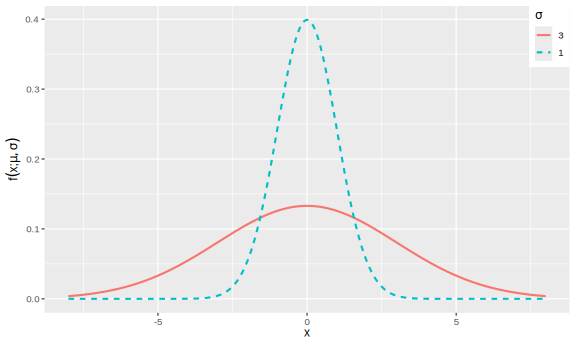
\includegraphics{01-sampling-distributions_files/figure-pdf/normals-diff-sd-1.pdf}

}

\caption{The pdfs of two normal rvs, \(X_1 \sim \mathsf{N}(0, 9)\) and
\(X_2 \sim \mathsf{N}(0, 1)\), with the same means and \emph{different
standard deviations}.}

\end{figure}%

\begin{definition}[Standard Normal
distribution]\protect\hypertarget{def-standard-normal}{}\label{def-standard-normal}

We say that \(X\) has a \textbf{standard normal distribution} if
\(\mu=0\) and \(\sigma = 1\) and we will usually denote standard Normal
rvs by \(Z \sim \mathsf{N}(0,1)\) (why \(Z\)? tradition!\footnote{``Traditions,
  traditions\ldots{} Without our traditions, our lives would be as shaky
  as a fiddler on the roof!''
  {[}\url{https://www.youtube.com/watch?v=gRdfX7ut8gw}{]}.}). We denote
the cumulative distribution function of the standard normal by
\(\Phi(z) = P(Z \leq z)\) and write \(\varphi = \Phi'\) for its density
function.

\end{definition}

\subsection{Some useful facts about normal
variates}\label{sec-facts-normals}

Here are some useful facts about how to manipulate Normal rvs.

\begin{enumerate}
\def\labelenumi{\arabic{enumi}.}
\tightlist
\item
  If \(X \sim \mathsf{N}(\mu, \sigma^2),\) then
  \(Z = (X - \mu) / \sigma  \sim \mathsf{N}(0,1).\)
\item
  If \(Z \sim \mathsf{N}(0, 1),\) then
  \(X = \mu + \sigma Z \sim \mathsf{N}(\mu, \sigma^2).\)
\item
  If \(X_i \sim \mathsf{N}(\mu_i, \sigma_i^2)\) for \(i = 1, \dots, n\)
  are independent rvs, then
  \[\sum_{i=1}^{n} X_i \sim \mathsf{N} \left( \sum_{i=1}^{n} \mu_i, \sum_{i=1}^{n} \sigma_i^2 \right) \,.\]
\end{enumerate}

In particular, we note that for differences of independent rvs
\(X_1 \sim \mathsf{N}(\mu_1, \sigma_1^2)\) and
\(X_2 \sim \mathsf{N}(\mu_2, \sigma_2^2)\) then the variances also add:
\[ X_1 - X_2 \sim \mathsf{N}(\mu_1 - \mu_2, \sigma_1^2 + \sigma_2^2) \,.\]

Probabilities \(P(a \leq X \leq b)\) are found by converting the problem
in \(X \sim \mathsf{N}(\mu, \sigma^2)\) to the \emph{standard normal}
distribution \(Z \sim \mathsf{N}(0, 1)\) whose probability values
\(\Phi(z) = P(Z\leq z)\) can then be looked up in a table. From (1.)
above, \[
\begin{aligned}
   P(a < X < b) &= P\left( \frac{a-\mu}{\sigma} < Z < \frac{b-\mu}{\sigma} \right) \\ 
    &= \Phi \left( \frac{b-\mu}{\sigma}\right) - \Phi\left(\frac{a-\mu}{\sigma}\right) \,.
\end{aligned}
\] This process is often referred to as \emph{standardising} (the normal
rv).

\begin{example}[]\protect\hypertarget{exm-norm-rt}{}\label{exm-norm-rt}

Let \(X \sim \mathsf{N}(5, 9)\) and find \(P(X \geq 5.5)\).

\[
\begin{aligned}
   P(X \geq 5.5) &= P\left(Z \geq \frac{5.5 - 5}{3}\right) \\
    &= P(Z \geq 0.1667) \\
    &= 1 - P(Z \leq 0.1667) \\
    &= 1 - \Phi(0.1667) \\
    &= 1 - 0.5662 \\
    &= 0.4338\,,
\end{aligned}
\] where we look up the value of \(\Phi(z) = P(Z\leq z)\) in a table of
standard normal curve areas.

The probability corresponds to the shaded area under the normal density
\(\varphi(x) = \Phi'(x)\) corresponding to \(x \geq 5.5\).

\begin{figure}[H]

{\centering 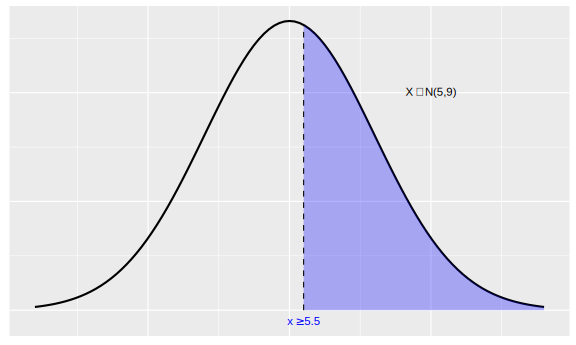
\includegraphics{01-sampling-distributions_files/figure-pdf/example-norm-geq-1.pdf}

}

\caption{The normal density from the exercise with the (one-sided)
interval shaded in blue.}

\end{figure}%

Alternatively, we can use the \texttt{r} code:
\texttt{pnorm(5.5,\ mean\ =\ 5,\ sd\ =\ 3,\ lower.tail\ =\ FALSE)}.

\end{example}

\begin{example}[]\protect\hypertarget{exm-norm-dt}{}\label{exm-norm-dt}

Let \(X \sim \mathsf{N}(5, 9)\) and find \(P(4 \leq X \leq 5.25)\).

\[
\begin{aligned}
   P(4 \leq X \leq 5.25) &= P\left(\frac{4-5}{3} \leq Z \leq \frac{5.25-5}{3}\right) \\
   &= P(-0.3333 \leq Z \leq 0.0833) \\
   &= \Phi(0.0833) - \Phi(-0.3333) \\
   &= 0.5332 - 0.3694 \\
   &= 0.1638\,.
  \end{aligned}
\] where we look up the value of \(\Phi(z) = P(Z\leq z)\) in a table of
standard normal curve areas.

The probability corresponds to the shaded area under the normal density
\(\varphi(x) = \Phi'(x)\) corresponding to \(4 \leq x \leq 5.25\).

\begin{figure}[H]

{\centering 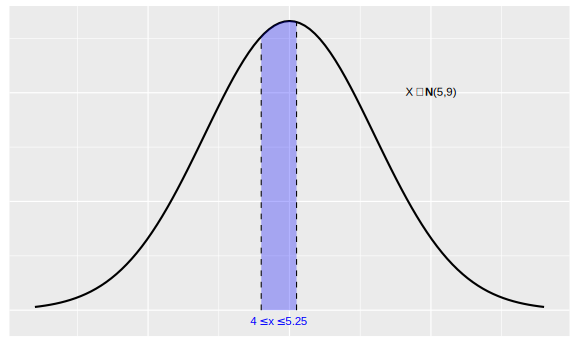
\includegraphics{01-sampling-distributions_files/figure-pdf/example-norm-interval-1.pdf}

}

\caption{The normal density from the exercise with the interval shaded
in blue.}

\end{figure}%

Alternatively, we can use the \texttt{r} code:
\texttt{pnorm(5.25,\ mean\ =\ 5,\ sd\ =\ 3)\ -\ pnorm(4,\ mean\ =\ 5,\ sd\ =\ 3)}.
\(\lozenge\)

\end{example}

\subsection{\texorpdfstring{Empirical rule (\(68-95-99.7\)
rule)}{Empirical rule (68-95-99.7 rule)}}\label{empirical-rule-68-95-99.7-rule}

For samples from a normal distribution, the percentage of values that
lie within one, two, and three standard deviations of the mean are
\(68.27\%\), \(95.45\%\), and \(99.73\%\), respectively. That is, for
\(X \sim \mathsf{N}(\mu, \sigma^2)\), \[
P(\mu - 1 \sigma \leq X \leq \mu + 1 \sigma ) \approx 0.6827\,,
\] \[
P(\mu - 2 \sigma \leq X \leq \mu + 2 \sigma ) \approx 0.9545\,,
\] \[
P(\mu - 3 \sigma \leq X \leq \mu + 3 \sigma ) \approx 0.9973\,.
\] For a normal population, nearly all the values lie within ``three
sigmas'' of the mean.

\section{\texorpdfstring{\(\mathsf{t}\) and Cauchy
distribution}{\textbackslash mathsf\{t\} and Cauchy distribution}}\label{t-distribution}

Student's \(\mathsf{t}\) distribution gets its peculiar name as it was
first published under the pseudonym ``Student''.\footnote{William Sealy
  Gosset (1876--1937) wrote under the pseudonym ``Student''
  {[}\url{https://mathshistory.st-andrews.ac.uk/Biographies/Gosset/}{]}.}
This bit of obfuscation was to protect the identity of his
employer,\footnote{Gosset invented the t-test to handle small samples
  for quality control in brewing, specifically for the Guinness brewery
  in Dublin {[}\url{https://www.wikiwand.com/en/Guinness_Brewery}{]}.}
and thereby vital trade secrets, in a highly competitive and lucrative
industry.

\begin{definition}[Student's
\(\mathsf{t}\)-distribution]\protect\hypertarget{def-t-dist}{}\label{def-t-dist}

A continuous rv \(X\) has a \textbf{\(\mathsf{t}\) distribution} with
parameter \(\nu > 0\), if \(X\) has pdf \begin{equation*}
f(x; \nu) = \frac{\Gamma\left(\tfrac{\nu+1}{2}\right)}{\sqrt{\nu \pi} \Gamma \left(\tfrac{\nu}{2}\right)} \left( 1 + \tfrac{x^2}{\nu} \right)^{- \frac{\nu+1}{2}} \,, \quad -\infty < x < \infty\,.
\end{equation*} We write \(X \sim \mathsf{t}(\nu)\). Note \(\Gamma\) is
the standard gamma function.\footnote{The gamma function is defined by
  \(\Gamma(z) = \int_0^\infty x^{z-1}e^{-x} dx\) when the real part of
  \(z\) is positive. For any positive integer \(n\),
  \(\Gamma(n) = (n-1)!\) and for half-integers
  \(\Gamma(\tfrac{1}{2} + n) = \frac{(2n)!}{4^n n!} \sqrt{\pi}\).}

\end{definition}

The density for \(\mathsf{t}(\nu)\) for several values of \(\nu\) are
plotted below.

\begin{figure}[H]

{\centering 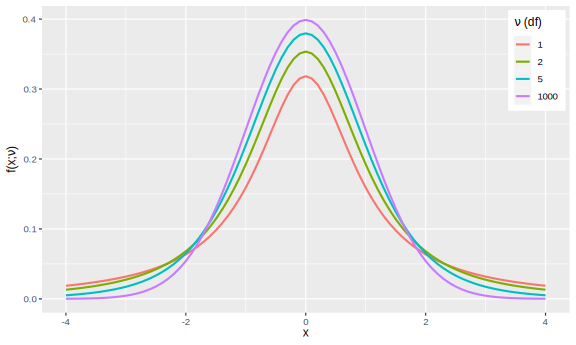
\includegraphics{01-sampling-distributions_files/figure-pdf/exemplar-t-dist-1.pdf}

}

\caption{The density for \(\mathsf{t}(\nu)\) for several values of
\(\nu\) (df).}

\end{figure}%

\begin{tipblock}
A \(\mathsf{t}\) distributions with \(\nu = 1\) has pdf
\[f(x) = \frac{1}{\pi (1 + x^2)}\,,\] and we call this the Cauchy
distribution.

\end{tipblock}

\subsection{\texorpdfstring{Properties of \(\mathsf{t}\)
distributions}{Properties of \textbackslash mathsf\{t\} distributions}}\label{facts-t}

\begin{enumerate}
\def\labelenumi{\arabic{enumi}.}
\tightlist
\item
  The density for \(\mathsf{t}(\nu)\) is a bell-shaped curve centred at
  \(0\).
\item
  The density for \(\mathsf{t}(\nu)\) is more spread out than the
  standard normal density (i.e., it has ``fatter tails'' than the
  normal).
\item
  As \(\nu \to \infty\), the spread of the corresponding
  \(\mathsf{t}(\nu)\) density converges to the standard normal density
  (i.e., the spread of the \(\mathsf{t}(\nu)\) density decreases
  relative to the standard normal).
\end{enumerate}

If \(X \sim \mathsf{t}(\nu)\), then \(\E[X] = 0\) for \(\nu > 1\)
(otherwise the mean is undefined).

\section{\texorpdfstring{\(\chi^2\)
distribution}{\textbackslash chi\^{}2 distribution}}\label{chisq-distribution}

The \(\chi^2\) distribution arises as the distribution of a sum of the
squares of \(\nu\) independent standard normal rvs.

\begin{definition}[\(\chi^2\)
distribution]\protect\hypertarget{def-chisq-dist}{}\label{def-chisq-dist}

A continuous rv \(X\) has a \textbf{\(\chi^2\) distribution} with
parameter \(\nu \in \mathbf{N}_{>}\), if \(X\) has pdf \begin{equation*}
f(x; \nu) = \frac{1}{2^{\nu/2} \Gamma(\nu/2)} x^{(\nu/2)-1} e^{-x/2} \,, 
\end{equation*} with support \(x \in (0, \infty)\) if \(\nu=1\),
otherwise \(x \in [0, \infty)\). We write \(X \sim \chi^2(\nu)\).

\end{definition}

The pdf \(f(x; \nu)\) of the \(\chi^2(\nu)\) distribution depends on a
positive integer \(\nu\) referred to as the df. The densities for
several values of \(\nu\) are plotted below.

\begin{figure}[H]

{\centering 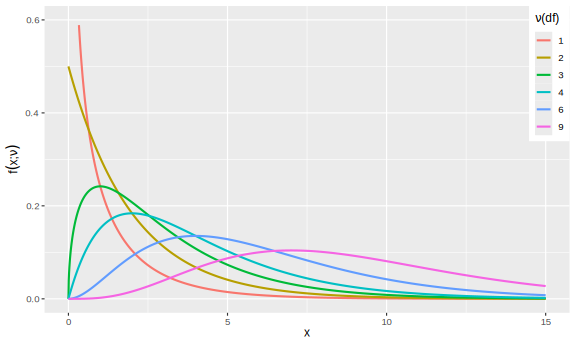
\includegraphics{01-sampling-distributions_files/figure-pdf/exemplar-chisq-dist-1.pdf}

}

\caption{The density for \(\chi^2(\nu)\) for several values of \(\nu\)
(df).}

\end{figure}%

The density \(f(x;\nu)\) is positively skewed, i.e., the right tail is
longer, so the mass is concentrated to the figure's left. The
distribution becomes more symmetric as \(\nu\) increases. We denote
critical values of the \(\chi^2(\nu)\) distribution by
\(\chi^2_{\alpha, \nu}\).

\begin{warningblock}
Unlike the normal and \(t\) distributions, the \(\chi^2\) distribution
is not symmetric. This means that the critical values
e.g.~\(\chi^2_{.99, \nu}\) and \(\chi^2_{0.01,\nu}\) are \textbf{not}
equal. Hence, it will be necessary to look up both values for CIs based
on \(\chi^2\) critical values.

\end{warningblock}

If \(X \sim \chi^2(\nu)\), then \(\E[X] = \nu\) and \(\Var[X] = 2\nu\).

\section{\texorpdfstring{\(\mathsf{F}\)
distribution}{\textbackslash mathsf\{F\} distribution}}\label{F-distribution}

The \(\mathsf{F}\) distribution (``F'' for Fisher) arises as a test
statistic when comparing population variances and in the analysis of
variance (see @ref(anova)).

\begin{definition}[\(\mathsf{F}\)
distribution]\protect\hypertarget{def-F-dist}{}\label{def-F-dist}

A continuous rv \(X\) has an \textbf{\(\mathsf{F}\) distribution} with
df parameters \(\nu_1\) and \(\nu_2\), if \(X\) has pdf \[
 f(x; \nu_1, \nu_2) = 
    \frac{\Gamma\left(\frac{\nu_1+\nu_2}{2}\right) \nu_1^{\nu_1/2} \nu_2^{\nu_2/2}}
 {\Gamma\left(\frac{\nu_1}{2}\right) \Gamma\left(\frac{\nu_2}{2}\right)} 
 \frac{x^{\nu_1/2 - 1}}{(\nu_2+\nu_1 x)^{(\nu_1+\nu_2)/2}} \,.
\]

\end{definition}

The pdf \(f(x; \nu_1, \nu_2)\) of the \(\mathsf{F}(\nu_1, \nu_2)\)
distribution depends on two positive integers \(\nu_1\) and \(\nu_2\)
referred to, respectively, as the numerator and denominator df. The
density is plotted below for several combinations of \((\nu_1, \nu_2)\).

\begin{figure}[H]

{\centering 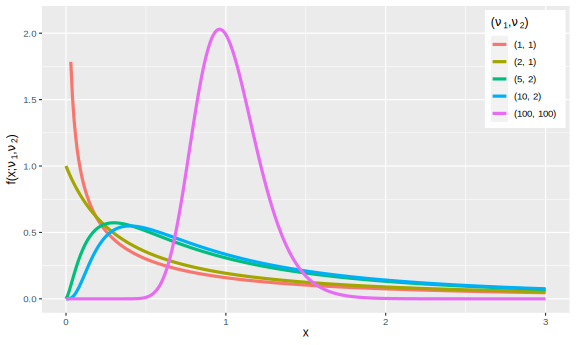
\includegraphics{01-sampling-distributions_files/figure-pdf/exemplar-F-dist-1.pdf}

}

\caption{The density for \(\mathsf{F}(\nu_1, \nu_2)\) for several
combinations of \((\nu_1, \nu_2)\).}

\end{figure}%

Where do the terms numerator and denominator df come from? The
\(\mathsf{F}\) distribution is related to ratios of \(\chi^2\) rvs.

\begin{theorem}[Ratio of \(\chi^2\)
rvs]\protect\hypertarget{thm-F-dist-chidq}{}\label{thm-F-dist-chidq}

If \(X_1 \sim \chi^2(\nu_1)\) and \(X_2 \sim \chi^2(\nu_2)\) are
independent rvs, then the rv \[
 F = \frac{X_1 / \nu_1}{X_2 / \nu_2} \quad \sim \mathsf{F}(\nu_1,\nu_2)\,,
\] that comprises the ratio of two \(\chi^2\) rvs divided by their
respective df has an \(\mathsf{F}(\nu_1, \nu_2)\) distribution.

\end{theorem}

\cleardoublepage
\phantomsection
\addcontentsline{toc}{part}{Appendices}
\appendix

\chapter*{Curated Content}\label{curated-content}
\addcontentsline{toc}{chapter}{Curated Content}

\markboth{Curated Content}{Curated Content}

Below we provide links to supplementary online material. Hopefully, some
of the items will inspire you to view the module material in a broader
context and lead to further investigations.

\section*{Investigation 0}\label{investigation-0}
\addcontentsline{toc}{section}{Investigation 0}

\markright{Investigation 0}

What is Statistics?

\begin{itemize}
\item
  \begin{description}
  \tightlist
  \item[Cambridge Ideas - Professor Risk]
  \url{https://www.youtube.com/watch?v=a1PtQ67urG4} \newline  Prof David
  Spiegelhalter (Cambridge University) discusses public understanding of
  risk. You may also be interested in reading
  (\citeproc{ref-Spiegelhalter:2020ps}{Spiegelhalter 2020}).
  \end{description}
\item
  \begin{description}
  \tightlist
  \item[The Joy of Statistics]
  \url{https://www.youtube.com/watch?v=jbkSRLYSojo} \newline  Prof Hans
  Rosling (Karolinska Institute and Gapminder Foundation) analyses data
  from 200 Countries over 200 Years in 4 Minutes - The Joy of Stats -
  BBC Four.
  \end{description}
\item
  \begin{description}
  \tightlist
  \item[Teach statistics before calculus!]
  \url{https://www.ted.com/talks/arthur_benjamin_teach_statistics_before_calculus}
  \newline  Prof Arthur Benjamin (Harvey Mudd College) argues that the
  pinnacle of math education is probability and statistics --- not
  calculus.
  \end{description}
\item
  \begin{description}
  \tightlist
  \item[Kaggle]
  \url{https://www.kaggle.com/} \newline Towards data science.

  \url{https://www.youtube.com/watch?v=TNzDMOg_zsw} \newline What's
  Kaggle?
  \end{description}
\end{itemize}

\section*{Investigation 1}\label{investigation-1}
\addcontentsline{toc}{section}{Investigation 1}

\markright{Investigation 1}

Defence against the dark arts.

\begin{itemize}
\item
  \begin{description}
  \tightlist
  \item[Three ways to spot bad statistics]
  \url{https://www.ted.com/talks/mona_chalabi_3_ways_to_spot_a_bad_statistic}
  \newline  Mona Chalabi (Data Journalist) discusses three ways to spot
  bad statistics.
  \end{description}
\end{itemize}

\begin{itemize}
\item
  \begin{description}
  \tightlist
  \item[Statistics Done Wrong]
  \url{https://www.statisticsdonewrong.com/} \newline  A book by Dr Alex
  Reinhart (Carnegie Mellon University).
  \end{description}
\item
  \begin{description}
  \tightlist
  \item[How to defend yourself against misleading statistics in the
  news]
  \url{https://www.youtube.com/watch?v=mJ63-bQc9Xg} \newline  Sanne
  Blauw (Journalist) discusses how the presentation of statistics can
  mislead.
  \end{description}
\end{itemize}

\section*{Investigation 2}\label{investigation-2}
\addcontentsline{toc}{section}{Investigation 2}

\markright{Investigation 2}

Data analysis and visualisation.

\begin{itemize}
\item
  \begin{description}
  \tightlist
  \item[The Grammar of Graphics]
  \url{https://www.youtube.com/watch?v=h-62NwWUI5c} \newline  What Makes
  A Good Visualisation? Rhys Jackson from RocketMill, a UK Digital
  Marketing Agency, gives a perspective on visualising data from a
  marketing perspective.

  \url{https://www.youtube.com/watch?v=kepKM7Z2O54} \newline  David
  Keyes (RStudio) discusses how the grammar of graphics underpins the
  \texttt{ggplot2} data visualization package in \texttt{R}.
  \end{description}
\item
  \begin{description}
  \tightlist
  \item[Same Stats, Different Graphs]
  \url{https://www.autodeskresearch.com/publications/samestats}
  \newline  Generating Datasets with Varied Appearance and Identical
  Statistics through Simulated Annealing (ACM SIGCHI Conference on Human
  Factors in Computing Systems) by Justin Matejka, George Fitzmaurice.
  \end{description}
\item
  \begin{description}
  \tightlist
  \item[Why do we so often use 0.05 for hypothesis testing?]
  \url{https://www.openintro.org/book/stat/why05/} \newline  In this
  online exercise, you will gain an improved understanding of what a
  significance level is, and why a value in the neighbourhood of 0.05 is
  reasonable as a default.
  \end{description}
\item
  \begin{description}
  \tightlist
  \item[Data visualisations]
  \url{https://flowingdata.com/} \newline  FlowingData blog by Nathan
  Yau.

  \url{https://fivethirtyeight.com/} \newline  FiveThirtyEight blog by
  Nate Silver.
  \end{description}
\item
  \begin{description}
  \tightlist
  \item[Storytelling with data]
  \url{http://www.storytellingwithdata.com/blog} \newline Blog with nice
  hints and tips for how to present data in tables, graphics, and
  visualisations.

  \url{https://community.storytellingwithdata.com/challenges}
  \newline Monthly challenge.
  \end{description}
\end{itemize}

\section*{Investigation 3}\label{investigation-3}
\addcontentsline{toc}{section}{Investigation 3}

\markright{Investigation 3}

Statistical paradoxes.

\begin{itemize}
\item
  \begin{description}
  \tightlist
  \item[How statistics can be misleading (TED-Ed)]
  \url{https://www.ted.com/talks/mark_liddell_how_statistics_can_be_misleading}
  \newline  Mark Liddell (Educator) discusses Simpson's Paradox in this
  TED-Ed animation.
  \end{description}
\item
  \begin{description}
  \tightlist
  \item[Low birth-weight paradox]
  \url{https://www.wikiwand.com/en/Low_birth-weight_paradox}
  \end{description}
\item
  \begin{description}
  \tightlist
  \item[Gambler's Fallacy]
  \url{https://www.youtube.com/watch?v=4eVluL-idkM} \newline  Prof Kelly
  Shue (Chicago Booth) discusses the gambler's fallacy.
  \end{description}
\end{itemize}

\section*{Investigation 4}\label{investigation-4}
\addcontentsline{toc}{section}{Investigation 4}

\markright{Investigation 4}

The law and interpreting statistics.

\begin{itemize}
\item
  \begin{description}
  \tightlist
  \item[How stats fool juries.]
  \url{https://youtu.be/kLmzxmRcUTo} \newline  Prof Peter Donnelly
  (Oxford University) discusses common mistakes in interpreting
  statistics.
  \end{description}
\item
  \begin{description}
  \tightlist
  \item[Better Data in Forensic Science]
  \url{https://www.dundee.ac.uk/leverhulme/projects/details/better-data-in-forensic-science.php}
  \newline  Dr Christian Cole (Dundee) is leading a data-focused project
  as part of the Leverhulme Research Centre for Forensic Science right
  here at Dundee.
  \end{description}
\item
  \begin{description}
  \tightlist
  \item[Prosecutor's fallacy]
  \url{https://www.wikiwand.com/en/Prosecutor\%27s_fallacy} \newline  A
  fallacy of statistical reasoning, typically used by a prosecutor to
  exaggerate the likelihood of guilt: because
  \(P(\text{hypothesis} \mid \text{evidence}) \neq P(\text{evidence} \mid \text{hypothesis})\)!
  \end{description}
\end{itemize}

\section*{Investigation 5}\label{investigation-5}
\addcontentsline{toc}{section}{Investigation 5}

\markright{Investigation 5}

Data-driven decision making in epidemiology.

\begin{itemize}
\item
  \begin{description}
  \tightlist
  \item[Project Tycho]
  \url{https://www.tycho.pitt.edu/} \newline  Digitized archival
  epidemiological data for the United States and the world.

  \url{https://www.youtube.com/watch?v=Kn9OJy1BPDo} \newline  An
  overview of the origins of project Tycho.
  \end{description}
\item
  \begin{description}
  \tightlist
  \item[Public Health Scotland COVID-19 Dashboard]
  \url{https://public.tableau.com/app/profile/phs.covid.19/viz/COVID-19DailyDashboard_15960160643010/Dailyupdate}
  \newline  The official COVID-19 dashboard of Public Health Scotland.
  \end{description}
\item
  \begin{description}
  \tightlist
  \item[Our World in Data]
  \url{https://ourworldindata.org/} \newline  A project of the Oxford
  Martin School to make public health data, including progress in UN
  Sustainable Development Goals, available and accessible.
  \end{description}
\item
  \begin{description}
  \tightlist
  \item[Demographic Party Trick]
  \url{https://www.youtube.com/watch?v=2nDh8MQuS-Y} \newline  Prof Hans
  Rosling (Karolinska Institute and Gapminder Foundation) and Bill Gates
  seek to shed light on the true statistics of childhood vaccinations.
  \end{description}
\end{itemize}

\section*{Investigation 6}\label{investigation-6}
\addcontentsline{toc}{section}{Investigation 6}

\markright{Investigation 6}

Spurious correlations!

\begin{itemize}
\item
  \begin{description}
  \tightlist
  \item[The danger of mixing up causality and correlation]
  \url{https://www.youtube.com/watch?v=8B271L3NtAw} \newline  Prov
  Ionica Smeets (University of Leiden) discusses causality and
  correlation.
  \end{description}
\item
  \begin{description}
  \tightlist
  \item[Spurious correlations]
  \url{https://tylervigen.com/spurious-correlations} \newline  Tyler
  Vigen's site dedicated to spurious correlations.
  \end{description}
\item
  \begin{description}
  \tightlist
  \item[Cause \& Effect]
  \url{https://www.youtube.com/watch?v=lbODqslc4Tg}
  \newline  Correlation vs.~causality from the Clip from the 2010
  documentary ``Freakonomics: The Movie''.
  \end{description}
\end{itemize}

\section*{Investigation 7}\label{investigation-7}
\addcontentsline{toc}{section}{Investigation 7}

\markright{Investigation 7}

Data and Society: can data-driven and predictive modelling lead to a
better world? What are the ethics of mass data collection?

\begin{itemize}
\item
  \begin{description}
  \tightlist
  \item[Science behind the news: Predictive Policing]
  \url{https://www.youtube.com/watch?v=74_jreara3w} \newline  The Los
  Angeles Police Department is using a new tactic in their fight against
  crime called ``predictive policing.'' It's a computer program
  originally developed by a team at UCLA, including mathematician Andrea
  Bertozzi and anthropologist Jeff Brantingham. ``Science Behind the
  News'' is produced in partnership with NBC Learn. (Provided by the
  National Science Foundation \& NBC Learn)
  \end{description}
\item
  \begin{description}
  \tightlist
  \item[You should get paid for your data]
  \url{https://www.nytimes.com/video/opinion/100000006678020/data-privacy-jaron-lanier-2.html}
  \newline  Jaron Lanier (Computer Scientist and Author) discusses a
  compensation plan and data dignity.

  \url{https://www.ted.com/talks/jennifer_zhu_scott_why_you_should_get_paid_for_your_data}
  \newline  Jennifer Zhu Scott (Computer Scientist) also thinks you
  should get paid for your data.
  \end{description}
\item
  \begin{description}
  \tightlist
  \item[How tech companies deceive you into giving up your data and
  privacy]
  \url{https://www.ted.com/talks/finn_lutzow_holm_myrstad_how_tech_companies_deceive_you_into_giving_up_your_data_and_privacy}
  \newline  Finn Lützow-Holm Myrstad (Norwegian Consumer Council)
  discusses consumer protections and data collection.
  \end{description}
\item
  \begin{description}
  \tightlist
  \item[Your company's data could help end world hunger]
  \url{https://www.ted.com/talks/mallory_freeman_your_company_s_data_could_help_end_world_hunger}
  \newline Mallory Freeman (Data Scientist) discusses how to do the most
  good with data.
  \end{description}
\end{itemize}

\section*{Investigation 8}\label{investigation-8}
\addcontentsline{toc}{section}{Investigation 8}

\markright{Investigation 8}

Machine learning / big data.

\begin{itemize}
\item
  \begin{description}
  \tightlist
  \item[What is Machine Learning?]
  \url{https://www.youtube.com/watch?v=f_uwKZIAeM0}
  \newline  OxfordSparks discusses the topic of supervised learning
  algorithms and how machine learning is used all around us.
  \end{description}
\item
  \begin{description}
  \tightlist
  \item[Big Data (TED-Ed)]
  \url{https://www.youtube.com/watch?v=j-0cUmUyb-Y} \newline Tim Smith
  (educator) discusses the historical arc of big data in this TED-Ed
  animation.
  \end{description}
\item
  \begin{description}
  \tightlist
  \item[The human insights missing from big data]
  \url{https://www.ted.com/talks/tricia_wang_the_human_insights_missing_from_big_data}
  \newline  Tricia Wang (Ethnographer) discusses the human insights
  missing from big data.
  \end{description}
\item
  \begin{description}
  \tightlist
  \item[How we can find ourselves in data]
  \url{https://www.ted.com/talks/giorgia_lupi_how_we_can_find_ourselves_in_data}
  \newline Giorgia Lupi (Designer) discusses a humanistic approach to
  data and data visualization.
  \end{description}
\end{itemize}

\phantomsection\label{refs}
\begin{CSLReferences}{1}{0}
\bibitem[\citeproctext]{ref-Spiegelhalter:2020ps}
Spiegelhalter, David J. 2020. \emph{The {A}rt of {S}tatistics:
{L}earning from {D}ata}. London: Pelican Books.

\end{CSLReferences}


\backmatter

\end{document}
